We now move to the formalities for the PRISM language. To the best of
our knowledge, the only formalisation of a semantics for PRISM can be
found on the PRISM website~\cite{prismemantics}. Our approach starts
from this and attempts to make more precise some informal assumptions
and definitions.

\smallskip

\mypar{Syntax.} In this section, we will reuse some of the syntactic
terms used for our choreography language, including assignments and
expressions. We define the syntax of (a subset of) the PRISM language
as follows:
\begin{displaymath}
  \begin{array}{lrlll@{\qquad}l}
    \text{(Networks)}  \quad
    & N, M  & ::=  &      & \CEnd & \text{empty network}\\
    &       &      & \mid & \role{p}:\{F_i\}_i & \text{module}\\
%    &       &      & \mid & M \pp M    & \text{parallel composition}\\
    &       &      & \mid & M \ppp A M & \text{parallel composition}\\
    % &       &      & \mid & M/A        & \text{action hiding}\\
    % &       &      & \mid & \sigma M   & \text{substitution}\\
    \\
    \text{(Commands)}  \quad
    & F     & ::=  &      & \command \alpha g\lambda u
                                  & \text{} (\alpha\in\{\epsilon\}\cup\mathcal L) \\
    % \\[1mm]
    % \text{(Assignment)} \quad
    % & u     & ::=  &      & (x' = E) & \text{update $x$ % , element of $\mathcal V$, 
    %                                    with $E$}\\
    % &       &      & \mid & u\ \&\ u   & \text{multiple assignments}
    % \\[1mm]
    % \text{(Expr)}\quad
    % & E, g     & ::= &       & f(\tilde E)\quad\mid\quad x\quad\mid\quad v & \text{expressions}
    % % \\[1mm]
    % % \text{(Rates)}\quad   &     \lambda\in\mathbb R
    % %  \\[1mm]
    % %   \text{(Variables)}\quad &   x\in\mathsf{Var} 
    % %  \\[1mm]
    % %   \text{(Values)}\quad     &  v\in\mathsf{Val} 
  \end{array}
\end{displaymath}
Networks are the top syntactic category for system of modules composed
together. The term $\CEnd$ represent an empty network. A module is
meant to represent a process running in the system, and is denoted by
its role name and its commands, formally written as
$\role{p}:\{F_i\}_i$, where $\role p$ is a role and $F_i$ are
commands. Networks can be composed in parallel, in a CSP style: a term
like $M_1 \ppp A M_2$ says that networks $M_1$ and $M_2$ can
synchronise using labels in the finite set $A$.
%
In this work, we omit PRISM hiding and substitution as they are
irrelevant for our current choreography language.
% The term $M/A$ is the standard CSP/CCS hiding operator. Finally
% $\sigma M$ is equivalent to applying the substitution $\sigma$ to
% all variables in $x$. A substitution is a function that given a
% variable returns a value. When we write $\sigma N$ we refer to the
% term obtained by replacing every free variable $x$ in $N$ with
% $\sigma(x)$. \marco{Is this really the way substitution is used?
% Where does it become important?}
%
Commands in a module have the form
$[\alpha] g \rightarrow \Sigma_{i\in I}\{\lambda_i: u_i\}$. The label
$\alpha$ can either be the empty string $\epsilon$ or a label $a$,
i.e., $\alpha\in\{\epsilon\}\cup \mathcal L$. If $\epsilon$ then no
synchronisation is required. On the other hand, if there is label $a$
then there will be a synchronisation with other modules that must
synchronise on $a$. The term $g$ is a guard on the current variable
state. If both label and guard are enabled, then the command executes
a branch $i$ with probability/rate $\lambda_i$. As for choreographies,
if the $\lambda_i$'s are probabilities, we must have that
$\Sigma_{i\in I}\lambda_i=1$.

\mypar{Semantics.} In order to give a probabilistic semantics to the
PRISM language, we follow the approach given in the PRISM
website~\cite{prismemantics}.  Hereby, we do that by defining two
relations: one with labels for networks and one on states. Our
relation on networks is the minimum relation $\prismred{}{}$
satisfying the rules given in Figure~\ref{fig:semantics}.
% 
\begin{figure}[h]
  \begin{displaymath}\small
    \begin{array}{ccc}
      \infer[\mathsf{(M)}]
      { {\role{p}:\{F_k\}_k} \prismred{} F
      % {\alpha}\lab{g}{\Sigma_{i\in I}\lambda_i\!}{u_i} 
      }
      {
      % \command {\alpha}g\lambda u
      F\in\{F_k\}_k
      }
      \quad
      \infer[\mathsf{(P_1)}]
      {M_1\ppp A M_2\prismred{}\command {\alpha}g\lambda u
      % {\alpha}\lab{g}{\Sigma_{i\in I}\lambda_i\!}{u_i}
      }
      {
      \exists j\in\{1,\!2\}.\ 
      M_j\prismred{} \command {\alpha}g\lambda u
      % {\alpha}\lab{g}{\Sigma_{i\in I}\lambda_i\!}{u_i}
      & \alpha\!\not\in\! A
        }
      \\\\
      \infer[\mathsf{(P_2)}]
      {M_1\ppp A M_2\prismred{}
      \commandBase a{g\land g'}
      {\Sigma_{i,j}\,\lambda_i*\lambda_j}: {u_i\& u_j} 
      }
      {
      M_1\prismred{}\command {\alpha}g\lambda u
      % {a}\lab{g}{\Sigma_{i\in I}\lambda_i}{\!u_i} 
      \quad&\quad 
        M_2\prismred{}\commandBase {\alpha} {g'} \Sigma_{j\in J}\lambda_j: u'_j
        % {a}\lab{g'}{\Sigma_{j\in J}\lambda'_j}{\!u'_j} 
      \ &\
             a\!\in\! A}
    \end{array}
  \end{displaymath}
  \caption{Semantics for PRISM networks} 
  \label{fig:semantics}
\end{figure}
Rule $\mathsf{(M)}$ just exposes a command at network level. Rule
$\mathsf{(P_1)}$ propagates a command through parallel composition if
$\alpha$ is empty or if the label $a$ is not part of the set $A$. When
the label $a$ is in $A$, we apply rule $\mathsf{(P_2)}$. In this case,
the product of the probabilities/rates must be taken by extending the
two different branches to every possible combination. 

Based on the relation above, given
$M\prismred{}\command \alpha g\lambda u$ and two
states $S$ and $S'$, we define the function
$$\mu(\command \alpha g\lambda u,\ S,\ S'\ ) = \Sigma_{S[u_i]=S',i\in I}\lambda_i$$
which gives the probability/rate for the system to go from state $S$
to state $S'$ after executing command $\command \alpha g \lambda u$,
for some $\alpha$.
%
If the $\lambda_i$ are probabilities, then the function must be a
probability distribution. Note that $\mu(F,S,S')$ only denotes the
probability/rate for the system to move from state $S$ to state $S'$
after executing command $F$. However, there could be several commands
derived from $M$ through the relation $\prismred{}$ that could be
executed to move from $S$ to $S'$. Therefore, we define the transition
relation on states $M\vdash S\red{\lambda}S'$ as
$$
\infer[\mathsf{(Transition)}]
{
  M\vdash S\red{\sum_{j} \mu(F_j,S,S')}S'
  % M\vdash S\red{\sum_{S'= S[u_j]} \lambda_j}S'
}
{
  \forall j,\alpha.\ M\prismred{}F_j
  % \command{\alpha_j} {g_j}{{\lambda_j}} {{u_j}}
  \quad&\quad
  S\vdash F_j
}
$$
where $S\vdash \command \alpha g\lambda u$ is defined as $\eval gS$.
Note that given the declarative aspect of the PRISM language, the
syntax is constant and never changes.

It is important to point out that, in general, the transition rule
above does not give the exact probability of a transition in case of a
Markov chain (DTMC), since the sum ${\sum_{j} \mu(F_j,S,S')}$ could be
a value greater than $1$. In order to get the right probability, the
value has to be normalised for all reachable $S'$. In the next
section, we will show that this is not an issue for networks that are
obtained from our translation from choreography to PRISM.

% At this point, we need to make a first observation about this
% construction whenever we are using probabilities [PUT NORMALISATION
% CONSTRAINT HERE].
% % Then, we define the transition relation $M\vdash S\red{\lambda}S'$ as
% % follows Note that if the $\lambda$'s are probabilities, hence, we deal
% % with an DTMC, then the probabilities of the branches outgoing from a
% % give state $S$ must be normalised -- this is because the sum at the
% % bottom of the $\mathsf{Transition}$ rule can be more than one. This is
% % not the case if we have a CTMC with rates.

\begin{example}
  Consider the following network $M$:
  \begin{displaymath}
    \begin{array}{llll}
      \role{p}: \{ & \quad \commandBase {}{x=0} {1:(x'=1)}\\
                   & \quad \commandBase {a}{y<1} {0.4: x'=x+1\ +\ 0.6: x'=x}\quad \}\\[2mm]
      \role{q}: \{ & \quad \commandBase {}{y=0} {1:(y'=1)}\\
                   & \quad \commandBase {a}{x<1} {0.5: y'=y+1\ +\ 0.5: y'=y}\quad \}\\
    \end{array}
  \end{displaymath}
  above, the two modules $\role p$ and $\role q$ can both do
  independent actions, as well as synchronising on label $a$. Applying
  the semantics, we can easily derive
  $M\prismred{}\commandBase {}{x=0} {1:(x'=1)}$,
  $M\prismred{}\commandBase {}{y=0} {1:(y'=1)}$, and, $M\prismred{}F$,
  such that
  \begin{displaymath}\small
    \begin{array}{rlll}
      F=\commandBase {a}{x<1\ \&\ y<1} {\quad} & 0.2: (x'=x+1)\ \&\ (y'=y+1)\\
                                       + & 0.2: (x'=x+1)\ \&\ (y'=y)\\
                                       + & 0.3: (x'=x)\ \&\ (y'=y+1)\\
                                       + & 0.3: (x'=x)\ \&\ (y'=y)\\
    \end{array}
  \end{displaymath}  
  Let $s_0=(x=0,y=0)$, $s_1=(x=1,y=0)$, $s_2=(x=0,y=1)$, and
  $s_0=(x=1,y=1)$ be all the possible states, with $s_0$ a starting
  state. Then,  we have that: 
  \begin{displaymath}
    \begin{array}{lr}
      \mu(\commandBase {}{x=0} {1:(x'=1)}, s_0, s_1) = 1 & \quad \mu(F, s_0, s_1) = 0.2\\
      \mu(\commandBase {}{y=0} {1:(y'=1)}, s_0, s_2) = 1 & \quad\mu(F, s_0, s_2) = 0.3\\ 
      \mu(F, s_0, s_0) = 0.3 & \quad\mu(F, s_0, s_3) = 0.2\\
    \end{array}
  \end{displaymath}  
  Now, by $\textsf{(Transition)}$, we have that
  $M\vdash s_0\rightarrow_{1.2} s_1$,
  $M\vdash s_0\rightarrow_{1.3} s_1$. Clearly, both transitions should
  be normalised, finally yielding the following DTMC:
\begin{comment}
  \begin{tikzpicture}\small
    \node[state, initial] (1) 
    {\tiny $s_0$};

    \node[state, below right of=1, xshift=1.5cm] (2) 
    {\tiny $s_1$};

    \node[state, above right of=1, xshift=1.8cm, yshift=0.5cm] (3) 
    {\tiny $s_2$};

    \node[state, right of=1, xshift=3.9cm] (4) 
    {\tiny $s_3$};

    \draw [->]  
    (1) edge[loop above] node{$0.3$} (1)
    (1) edge[above, bend right] node{$1.2$} (2)
    (1) edge[above, bend left] node{$1.3$} (3)
    (1) edge[above] node{$0.2$} (4)
    (2) edge[below, bend right] node{$1$} (4)
    (3) edge[below, bend left] node{$1$} (4)
    ;
  \end{tikzpicture} {\color{red}{[We must not forget to normalise probabilities and
  make the diagram prettier]}}
\end{comment}
\begin{figure}[h]
  \centering
  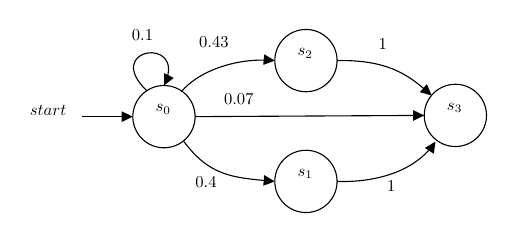
\begin{tikzpicture}[x=0.75pt,y=0.75pt,yscale=-1,xscale=1,scale=0.6, every node/.style={scale=0.6}]
    %uncomment if require: \path (0,300); %set diagram left start at 0, and has height of 300
    
    %Straight Lines [id:da5827855411335001] 
    \draw    (92,121) -- (130,121) ;
    \draw [shift={(133,121)}, rotate = 180] [fill={rgb, 255:red, 0; green, 0; blue, 0 }  ][line width=0.08]  [draw opacity=0] (8.93,-4.29) -- (0,0) -- (8.93,4.29) -- cycle    ;
    %Shape: Circle [id:dp9219571062705167] 
    \draw   (133,121) .. controls (133,107.19) and (144.19,96) .. (158,96) .. controls (171.81,96) and (183,107.19) .. (183,121) .. controls (183,134.81) and (171.81,146) .. (158,146) .. controls (144.19,146) and (133,134.81) .. (133,121) -- cycle ;
    %Shape: Circle [id:dp6656955165501577] 
    \draw   (247,76) .. controls (247,62.19) and (258.19,51) .. (272,51) .. controls (285.81,51) and (297,62.19) .. (297,76) .. controls (297,89.81) and (285.81,101) .. (272,101) .. controls (258.19,101) and (247,89.81) .. (247,76) -- cycle ;
    %Shape: Circle [id:dp8334106106935677] 
    \draw   (247,173) .. controls (247,159.19) and (258.19,148) .. (272,148) .. controls (285.81,148) and (297,159.19) .. (297,173) .. controls (297,186.81) and (285.81,198) .. (272,198) .. controls (258.19,198) and (247,186.81) .. (247,173) -- cycle ;
    %Shape: Circle [id:dp8330211202457276] 
    \draw   (367,120) .. controls (367,106.19) and (378.19,95) .. (392,95) .. controls (405.81,95) and (417,106.19) .. (417,120) .. controls (417,133.81) and (405.81,145) .. (392,145) .. controls (378.19,145) and (367,133.81) .. (367,120) -- cycle ;
    %Straight Lines [id:da2039531722214365] 
    \draw    (183,121) -- (364,120.02) ;
    \draw [shift={(367,120)}, rotate = 179.69] [fill={rgb, 255:red, 0; green, 0; blue, 0 }  ][line width=0.08]  [draw opacity=0] (8.93,-4.29) -- (0,0) -- (8.93,4.29) -- cycle    ;
    %Curve Lines [id:da5000591101938383] 
    \draw    (172,101) .. controls (183.64,86.45) and (212.22,73.78) .. (244.04,75.77) ;
    \draw [shift={(247,76)}, rotate = 185.19] [fill={rgb, 255:red, 0; green, 0; blue, 0 }  ][line width=0.08]  [draw opacity=0] (8.93,-4.29) -- (0,0) -- (8.93,4.29) -- cycle    ;
    %Curve Lines [id:da15038978821612803] 
    \draw    (297,76) .. controls (339.02,75.05) and (355.5,88.68) .. (370.84,102.11) ;
    \draw [shift={(373,104)}, rotate = 221.19] [fill={rgb, 255:red, 0; green, 0; blue, 0 }  ][line width=0.08]  [draw opacity=0] (8.93,-4.29) -- (0,0) -- (8.93,4.29) -- cycle    ;
    %Curve Lines [id:da2693493771645583] 
    \draw    (174,141) .. controls (194.48,168.3) and (212.1,169.93) .. (244.48,172.78) ;
    \draw [shift={(247,173)}, rotate = 185.04] [fill={rgb, 255:red, 0; green, 0; blue, 0 }  ][line width=0.08]  [draw opacity=0] (8.93,-4.29) -- (0,0) -- (8.93,4.29) -- cycle    ;
    %Curve Lines [id:da966786277015226] 
    \draw    (297,173) .. controls (323.19,173.97) and (356.91,167.41) .. (374.42,143.29) ;
    \draw [shift={(376,141)}, rotate = 123.18] [fill={rgb, 255:red, 0; green, 0; blue, 0 }  ][line width=0.08]  [draw opacity=0] (8.93,-4.29) -- (0,0) -- (8.93,4.29) -- cycle    ;
    %Curve Lines [id:da8313978097276571] 
    \draw    (144,100) .. controls (108.72,65.7) and (175.24,56.37) .. (159.09,93.66) ;
    \draw [shift={(158,96)}, rotate = 296.57] [fill={rgb, 255:red, 0; green, 0; blue, 0 }  ][line width=0.08]  [draw opacity=0] (8.93,-4.29) -- (0,0) -- (8.93,4.29) -- cycle    ;
    
    % Text Node
    \draw (49,111) node [anchor=north west][inner sep=0.75pt]   [align=left] {$\displaystyle start$};
    % Text Node
    \draw (150,110) node [anchor=north west][inner sep=0.75pt]   [align=left] {$\displaystyle s_{0}$};
    % Text Node
    \draw (264,65) node [anchor=north west][inner sep=0.75pt]   [align=left] {$\displaystyle s_{2}$};
    % Text Node
    \draw (264,162) node [anchor=north west][inner sep=0.75pt]   [align=left] {$\displaystyle s_{1}$};
    % Text Node
    \draw (384,109) node [anchor=north west][inner sep=0.75pt]   [align=left] {$\displaystyle s_{3}$};
    % Text Node
    \draw (131,50) node [anchor=north west][inner sep=0.75pt]   [align=left] {$\displaystyle 0.1$};
    % Text Node
    \draw (185,56) node [anchor=north west][inner sep=0.75pt]   [align=left] {$\displaystyle 0.43$};
    % Text Node
    \draw (182,168) node [anchor=north west][inner sep=0.75pt]   [align=left] {$\displaystyle 0.4$};
    % Text Node
    \draw (205,101) node [anchor=north west][inner sep=0.75pt]   [align=left] {$\displaystyle 0.07$};
    % Text Node
    \draw (329,57) node [anchor=north west][inner sep=0.75pt]   [align=left] {$\displaystyle 1$};
    % Text Node
    \draw (336,171) node [anchor=north west][inner sep=0.75pt]   [align=left] {$\displaystyle 1$};
    
    \end{tikzpicture}
\end{figure}
\end{example}

% SEMANTICS WITH GUESS (Early)
%
% \begin{figure}[t]
%   \begin{displaymath}\small
%     \begin{array}{ccc}
%       \infer[\mathsf{(M_1)}]
%       { {\role{p}:\{F_k\}_k} \prismred{}\lab{g}{\lambda_i}{u_i} }
%       {\command {}g\lambda u\in\{F_k\}_k}
%       \qquad
%       \infer[\mathsf{(P_1)}]
%       {M_1\ppp A M_2\prismred{\alpha}\lab g\lambda u }
%       {
%       \exists j\in\{1,2\}.\ 
%       M_j\prismred{\alpha}\lab g\lambda u
%       & \alpha\not\in A
%         }
%       \\\\
%       \infer[\mathsf{(M_2)}]
%       { {\role{p}:\{F_k\}_k} \prismred{a}\lab{g}{\lambda_i\!\!}{u_i} }
%       {\command ag\lambda u\in\{F_k\}_k}
%       \quad
%       \infer[\mathsf{(P_2)}]
%       {M_1\ppp A M_2\prismred{a}\lab{g_1\land g_2}{\lambda_1*\lambda_2\!\!}{u_1\& u_2} }
%       {
%       M_1\!\!\!\prismred{a}\!\!\!\lab{g_1}{\lambda_1\!\!}{\!\!u_1} 
%       & M_2\!\!\!\prismred{a}\!\!\!\lab{g_2}{\lambda_2\!\!}{\!\!u_2} 
%       & a\!\in\! A}
%     \end{array}
%   \end{displaymath}
%   \caption{LTS for PRISM networks} 
%   \label{fig:semantics}
% \end{figure}

%%% Local Variables: 
%%% mode: latex
%%% TeX-master: "main"
%%% End: